
\subsection{Automatic User Preference Gathering}

User profiles are a virtual representation of a user
containing their characteristics~\cite{Cufoglu}. In
addition, some tourist planners make use of such a
technique to personalise the results of their
system~\cite{Worndl2017, Lim2018a, Tumas2009,
Gavalas2015}. For example, Wörndl et al.
\cite{Worndl2017} required the upcoming tourists to
input their preferences manually by rating six
categories on a scale of 0 to 5: \textit{Sights and Museums,
Night Life, Food, Outdoors and Recreation
 and Shopping}. Including a manual input of user
preferences resulted in high user satisfaction since
their timetable was very customised.

\subsubsection{Automatic preference gathering in Travel Planning Applications}

In 2018, Lim et al.\cite{Lim2018a} demonstrated how
implementing personalisation in their algorithm,
PersTours, helped portray real-life scenarios more
accurately. The authors built a system where the
tourist’s level of interest in a specific category is
dependant on their time spent at such POIs, relative
to the average user. First, they gathered information
from the user’s past trips from the social media
platform Flickr. Then, they evaluated their algorithm
using the Root-Mean-Square Error (RMSE), representing
the time deviation of past trips and PersTours results
from Flickr. Although their results show the PersTours
outperforms other applications that use
frequency-based user interest, this approach requires
users to use Flickr and post information about their
past trips on the platform.
 
Nguyen et al.\cite{Nguyen2018} developed an Android
chat application called STSGroup that gathers user’s
preferences and resolves conflicts between tourists by
understanding the messages sent in a group chat. They
provided an example of students travelling to South
Tyrol (Italy), which gathered information such as the
users’ mood and recommended POIs from their
conversations. Other users in the group chat rate
their suggestions through a voting system as the
system uses raking and logistics to calculate
the ideal group preferences in the background. As a
result, 86.7\% of the test users showed satisfaction
with the suggestions.  

\subsubsection{Automatic preference gathering through social media}

The average internet user has gone from being a
passive content absorber to a content producer through
social media. TTDP solutions can use this advantage
and provide a fully automated activity plan based on
the user's characteristics. The following are some
methods for user profiling and information gathering
from the user's social media. 


Instagram has a significant effect on the tourism
industry. Sharing photos of amazing sights and
landscapes influence the way people choose their
POIs\cite{Terttunen2017}. Therefore, a system that
uses tourist's social media photos could infer the
user's preference.

Guntuku et al.~\cite{Guntuku2017} performed an
analysis on the relationship between a user's
characteristics and online images. They found that the
media on the social media profile can predict the big
five personality traits; conscientiousness,
extraversion, neuroticism, agreeableness and openness.
The performance graded by the Pearson correlations
tests were 0.530 and 0.566 for prognosticating
neuroticism and conscientiousness, respectively.

Chen et al.\cite{Chen2013} produced a system for
automatically retrieving tags from images and
incomplete tags called \emph{FastTag}. The algorithm
uses two simple linear mappings. Figure ~\ref{fasttag}
shows an example of an input image used alongside the
tags \emph{snow, lake, and feet}. In addition, the algorithm produced the
 tags; \emph{mountain, water, legs, boat,
trees}. 


\begin{figure}[h]
\centering
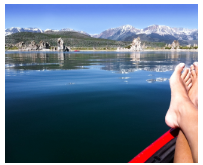
\includegraphics[width=0.4\textwidth]{Fastag}
\caption{Example of an image input for the FastTag algorithm}
\label{fasttag}
\end{figure}

These approaches show how image classification
techniques could provide an automatic preference
gathering system.
